\section{Railway Signaling Basics}

\label{sec:literature:signaling-basics}

Railway signaling forms the backbone of operational safety in rail networks. It governs train movements, enforces safe separation, and controls access to sections of track through structured signal aspects and interlocking logic.

Traditional signaling systems rely on the concept of fixed blocks—sections of track that can only be occupied by a single train at a time. These systems use a variety of signal types:

Mechanical Signals: These are the earliest form of railway signaling, relying on physical arms, discs, or semaphores that are moved into position by levers, pulleys, or rod linkages. Mechanical signals are usually operated manually from a signal cabin, where a signaller physically sets the route. Their visibility depends on daylight and line-of-sight conditions, which makes them less effective in poor weather or long-distance operations. While robust and historically reliable, mechanical signals require intensive maintenance due to the wear and tear of moving parts, and they limit the scalability of railway operations in high-density environments.

Color Light Signals: With the advent of electricity, color light signals replaced mechanical semaphores in many modern systems. These signals use combinations of colored lights—typically red, yellow, and green—to indicate movement authority to drivers. Unlike mechanical systems, they allow longer visibility at night and in adverse weather, and can be integrated with track circuits or axle counters to automatically reflect the state of track occupancy. Color light systems also enable more complex aspects (e.g., flashing indications for speed restrictions), allowing finer control over train movements. However, they still depend on fixed-block principles, which can restrict capacity on congested corridors, and their reliance on electrical infrastructure increases susceptibility to power failures or equipment faults.

Cab Signaling: Cab signaling advances beyond trackside signals by transmitting movement authority directly into the driver’s cab. This system uses track-to-train communication—either via track circuits, balises, or radio transmission—to continuously inform the driver of speed limits, upcoming restrictions, or route clearance. By reducing reliance on external visual cues, cab signaling enhances safety in poor visibility and allows for more dynamic train control. In advanced implementations such as the European Train Control System (ETCS), cab signaling forms the foundation for moving block operations, significantly increasing capacity and operational flexibility. However, implementation costs are higher, and successful deployment requires compatibility between onboard equipment and trackside infrastructure.

\noindent The following figures illustrate the three main signaling types:

\begin{figure}[t]
    \centering

    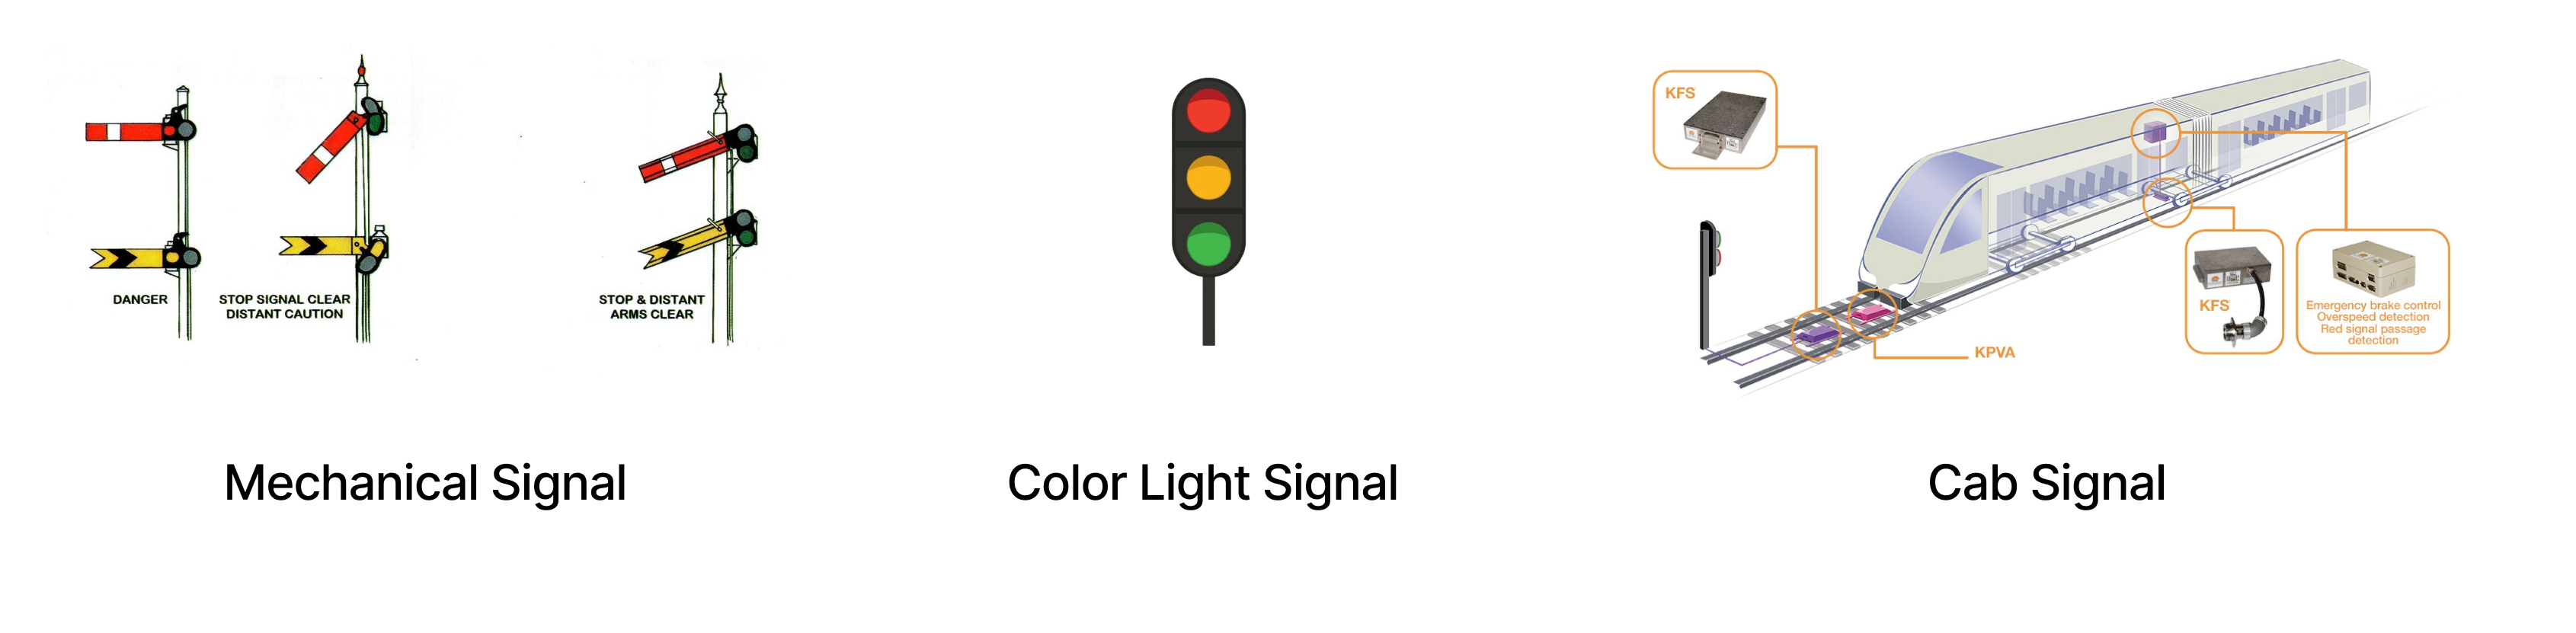
\includegraphics[width=1\textwidth]{images/signal-types/signalling_types.png}

    \floatcap{Different Signals}{Signals from left to right: Mechanical Signals, Color Light Signals, Cab Signal}
    
    \label{fig:signalling-types}
\end{figure}

While these mechanisms ensure safety, they often lack adaptability to real-time operational dynamics, especially in complex junctions or high-density corridors.